\documentclass[9.5pt]{beamer}

\mode<presentation>
{
  \usetheme{Warsaw}       % or try default, Darmstadt, Warsaw, ...
  \usecolortheme{default} % or try albatross, beaver, crane, ...
  \usefonttheme{serif}    % or try default, structurebold, ...
  \setbeamertemplate{navigation symbols}{}
  \setbeamertemplate{caption}[numbered]
} 

\usepackage[utf8]{inputenc} % accents 8 bits dans le fichier
\usepackage[T1]{fontenc}      % accents codés dans la fonte
\usepackage[french]{babel}
\usepackage{amsmath,amssymb}
\usepackage{graphicx}
\usepackage{fancyhdr}
\usepackage{siunitx}
\usepackage[mode=buildnew]{standalone}
\usepackage{algorithmicx}
\usepackage{algorithm}
\usepackage{algpseudocode}


% Here's where the presentation starts, with the info for the title slide
\title[MPNA : MIS]{Présentation AOC \\Application MiniMD}
\author[\bsc{Beaupère} \& \bsc{Granger}]{Matthias \bsc{Beaupère} \& Pierre \bsc{Granger}}
\institute{M2 CHPS}
\date{\today}

\begin{document}
\setbeamercolor{captioncolor}{fg=white,bg=red!80!white}
\setbeamertemplate{caption}{%
\begin{beamercolorbox}[wd=0.8\linewidth, sep=.2ex]{captioncolor}\tiny\centering\insertcaption%
\end{beamercolorbox}%
}

\begin{frame}
  \titlepage
\end{frame}

\begin{frame}{Plan}
	\tableofcontents[hideallsubsections]
\end{frame}

\section{Présentation de la dynamique moléculaire}
	\begin{frame}{Présentation de la dynamique moléculaire}
	\end{frame}

\section{Présentation de l'application}
	\begin{frame}{Présentation de l'application}
	\end{frame}

	\begin{frame}{Utilisation de l'application}
		Compilation + test + lancement en général
	\end{frame}

\section{Etude de performances}
	\subsection{Cadre d'expérimentation}
		\begin{frame}{Matériel}
			\begin{block}{Processeur et mémoire vive}
				\begin{itemize}
					\item Intel Core i5-760 2.80GHz (2011)
					\item 2 c\oe{}urs physiques (4 logiques)
					\item 8Go DDR3
				\end{itemize}
			\end{block}

			\begin{block}{Micro-architecture}
				\begin{itemize}
					\item Nehalem
					\item SSE 4.2 $\rightarrow$ vecto sur 128 bits
				\end{itemize}
			\end{block}
		\end{frame}

		\begin{frame}{Compilation}
			\begin{block}{Compilateur et options}
				\begin{itemize}
					\item GCC 5.4
					\item \verb!-Ofast!
					\item \verb!--funroll-loops!
					\item \verb!-g!
				\end{itemize}
			\end{block}
		\end{frame}

		\begin{frame}{Exécution et profiling}
			\begin{block}{Paramétrage de miniMD}
				\begin{itemize}
					\item Taille du problème 64 x 64 x 64
					\item Densité 0.8 $\rightarrow 10^6$ atomes
					\item 4 threads OpenMP
					\item 1 processus MPI
					\item timestep 5 ms
					\item durée de simulation 0.5s
				\end{itemize}
			\end{block}
		\end{frame}

	\subsection{Résultats}
		\begin{frame}{Etude générale}
			
			\begin{figure}[h!]
				\centering
				\begin{center}
					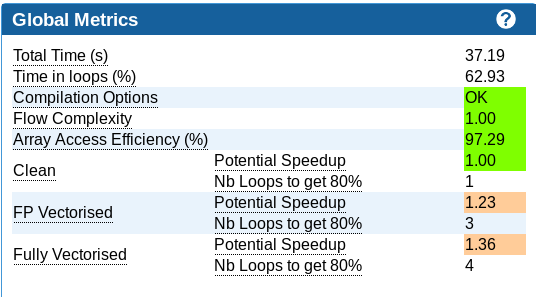
\includegraphics[width=200px]{images/maqao_global_metrics.png}
					\caption{Métriques global obtenu avec Maqao pour 4 threads}
					\label{global_maqao}
				\end{center}
			\end{figure}
		\end{frame}

		\begin{frame}{Etude générale}
			
			\begin{figure}[h!]
				\centering
				\begin{center}
					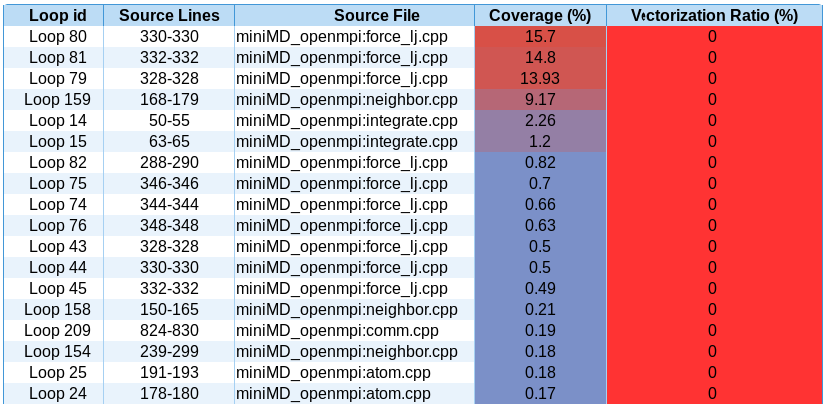
\includegraphics[width=300px]{images/maqao_loops.png}
					\caption{Statistiques des boucles obtenu avec Maqao pour 4 threads}
					\label{loop_maqao}
				\end{center}
			\end{figure}
		\end{frame}

		\begin{frame}{Analyse des points chauds}
			
		\end{frame}

\section{Optimisations}
	\subsection{Tentatives d'optimisation}
		\begin{frame}{Tentatives d'optimisation}
		\end{frame}

	\subsection{Optimisations envisageables}
		\begin{frame}{Vectorisation explicite}
		\end{frame}

\section{Analyse du parallélisme}
	\begin{frame}{Analyse du parallélisme}
	\end{frame}

\section{Conclusion}
	\begin{frame}{Conclusion}
	\end{frame}

\end{document}
